%xelatex -shell-escape -output-directory=bin ergasia.tex
\documentclass{assignment}


\usepackage{pdflscape}
\usepackage{enumerate} % Για την χρησιμοποίηση roman enumerate
\usepackage{paralist} % για το περιβάλλον inparaenum που είναι οι λίστες μέσα στο κείμενο.

\title{Πληροφοριακό σύστημα για online πωλήσεις της εταιρείας ΒΙΒΛΙΟΠΟΛΕΙΟ Α.Ε.}
\date{Αθήνα, 2015}

\author{Αναγνωστόπουλος Βασίλης - Θάνος (ΜΠΠΛ 13002) \\
        Βιδάλης Γιάννης (ΜΠΠΛ 13\_\_\_) \\
        Λιόλης Γιώργος  (ΜΠΠΛ 13\_\_\_) \\
        Χρόνη Ειρήνη    (ΜΠΠΛ 13\_\_\_)  }

\begin{document}

\maketitle
% Να σκεφτώ τί αλλαγές θέλω να κάνω με τις αριθμήσεις και άμα θέλω να κάνω.
% Να σκεφτώ να τις ενσωματώσω και στο assignment.cls

\setcounter{page}{1} 
\pagenumbering{roman}

\pagestyle{plain}
\tableofcontents
%\listoftables
\listoffigures
%\renewcommand\listoflistingscaption{Κατάλογος πηγαίου κώδικα}
%\listoflistings
\newpage

%\pagestyle{headings}
%\pagestyle{fancy}
\setcounter{page}{1} 
\pagenumbering{arabic}

\section{Εισαγωγή}

Η εργασία αυτή έχει ως σκοπό την σχεδίαση και ανάλυση ενός πληροφοριακός συστήματος. Συγκεκριμένα η παρούσα αναφορά περιγράφει την βασική λειτουργικότητα και τις σχεδιαστικές αποφάσεις που αφορούν την υλοποίηση του Πληροφοριακού Συστήματος (Π.Σ.) για την \emph{ΤΙ ΑΚΡΙΒΩΣ ΒΑΖΟΥΜΕ ;;;;;;} . Θα παρουσιαστούν οι λειτουργικές και οι μη λειτουργικές απαιτήσεις του συστήματος, το περιβάλλον το οποίο θα χρησιμοποιείται καθώς και οι χρήστες του. Στην συνέχεια θα γίνει μοντελοποίηση του συστήματος με την βοήθεια διαγραμμάτων των διαγραμμάτων κλάσεων, διαγραμμάτων ροής και περιπτώσεων χρήσης και έπειτα θα ακολουθήσει η υλοποίηση του συστήματος.

\subsection{Περιβάλλον του έργου}

%Θα πρέπει να προσδιοριστούν οι στόχοι που θα υλοποιηθούν από το σύστημα, οι προδιαγραφές που θα έχει και οι περιορισμοί στους οποίους θα πρέπει να συμμορφώνεται. Θα πρέπει επίσης να διασφαλιστεί ότι θα ικανοποιηθούν οι ανάγκες των ενδιαφερόμενων και για να γίνει αυτό θα πρέπει να οριστούν με ακρίβεια οι λειτουργικές και οι μη λειτουργικές απαιτήσεις.

% Το περιβάλλον περιγράφει την εταιρεία και ο σκοπός είναι για ποιον λόγο δημιουργείται.

Η εταιρεία "ΒΙΒΛΙΟΠΟΛΕΙΟ Α.Ε.", που από εδώ και πέρα απλώς θα καλείται "εταιρεία", δραστηριοποιείται πώληση βιβλίων. Η εταιρεία αναπτύσσει την επιχειρηματική της δραστηριότητα σύμφωνα με την ελληνική νομοθεσία που διέπει της ανώνυμες εταιρείες.

Βασικός σκοπός της εταιρείας είναι:

\begin{itemize}
\item Η προώθηση βιβλίων από τους εκδοτικούς οίκους. 
\item ΝΑ ΣΚΕΦΤΟΥΜΕ ΚΑΙ ΤΠΤ ΑΛΛΟ !!!
\end{itemize}


\subsection{Περιγραφή του προβλήματος και των εναλλακτικών λύσεων}

Η εταιρεία "ΒΙΒΛΙΟΠΟΛΕΙΟ Α.Ε." επιθυμεί την ανάπτυξη πληροφοριακού συστήματος για την κάλυψη των αναγκών της. Το πληροφοριακό αυτό σύστημα θα πρέπει να καλύπτει τόσο τις ανάγκες της εσωτερικής της λειτουργίας (διαχείριση αγορών και πωλήσεων, κ.λ.π.), όσο και την πώληση βιβλίων μέσω του διαδικτύου.

Με την διείσδυση των νέων τεχνολογιών στην καθημερινότητα, οι άνθρωποι χρησιμοποιούν όλο και περισσότερο το διαδίκτυο για την πραγματοποίηση απλών καθημερινών διαδικασιών. Παρά το γεγονός ότι η χρήση του internet παραμένει χαμηλή στη Ελλάδα συγκριτικά με την Ευρώπη, σχεδόν ένας στους πέντε Έλληνες (ποσοστό 20,08\%) χρησιμοποιεί πια το διαδίκτυο, ενώ το 17,9\% του πληθυσμού το χρησιμοποιεί τακτικά τουλάχιστον μια φορά την εβδομάδα. Οι νεαρότερες ηλικιακά ομάδες (16-24 ετών: 42\%, 25-34 ετών: 30\%) και οι κάτοικοι των αστικών πόλεων με ανώτερη μόρφωση, αποτελούν με σημαντική διαφορά τις ομάδες πληθυσμού με την υψηλότερη πρόσβαση \cite{infosoc}. 

Βασισμένοι στα παραπάνω, η εταιρεία θεωρεί σημαντικό για την προώθηση των θερινών κινηματογράφων να αναπτυχθεί ένα σύστημα λογισμικού για την πώληση βιβλίων μέσω διαδικτύου.

\subsection{Σκοπός και στόχος του Π.Σ.}

Σκοπός της συγκεκριμένης μελέτης είναι η υλοποίηση ενός Π.Σ. που αποσκοπεί στην προώθηση ... %. Ακόμα μέσω του Π.Σ. θα είναι δυνατή η κράτηση θέσεων μέσω του διαδικτύου και η αποπληρωμή των εισιτηρίων με ηλεκτρονικούς τρόπους πληρωμής (π.χ. πιστωτικές κάρτες, paypal, κ.λ.π.), προσφέροντας με αυτό τον τρόπο ένα εναλλακτικό τρόπο αγοράς των εισιτηρίων για τους κινηματογράφους. Το Π.Σ. αναμένεται να αποφέρει οφέλη στους τομείς:

\begin{itemize}
\item της διαφήμισης, μίας και η ιστοσελίδα για την πώληση των βιβλίων των θέσεων θα αποτελεί και ταυτόχρονα μέσω προώθησης της εταιρείας
%\item της εξυπηρέτησης των πελατών, μίας και οι πελάτες δεν θα πρέπει να περιμένουν στην σειρά για την απόκτηση θέσης και θα έχουν την δυνατότητα να αγοράζουν το εισιτήριο τους από όπου θέλουν.
%\item της οργάνωσης της εταιρείας, μίας και θα δημιουργηθεί ένα αυτόματο σύστημα επεξεργασίας της διαθεσιμότητας των θέσεων
%\item μείωση κόστους και αύξηση του κέρδους, μίας και θα μειωθούν οι εργαζόμενοι οι οποίοι βρίσκονται στους κινηματογράφους για να κόβουν εισιτήρια. 
\item ΝΑ ΣΚΕΦΤΟΥΜΕ ΚΑΙ ΤΠΤ ΑΛΛΟ !!!
\end{itemize}

Η επιτυχία του έργου θα κριθεί κυρίως από το εύρος χρήσης του και από την αξιοποίηση των εξειδικευμένων δυνατοτήτων του, που αποσκοπούν κύρια στην αυτοματοποίηση του συστήματος για την κράτηση θέσεων.

Μετά την ολοκλήρωση του έργου του Π.Σ. θα ωφεληθούν άμεσα:

\begin{itemize}
\item οι πελάτες της εταιρεία, μίας και δεν χρειάζεται πλέον να περιμένουν στην σειρά για να πάρουν το βιβλίο τους, 
%\item οι εργαζόμενοι της εταιρείας μίας και θα απλοποιηθεί η διαδικασία για την κράτηση θέσεων
%\item και οι θερινοί κινηματογράφοι της εταιρείας μίας και θα έχουν έναν εύκολο τρόπο να διαφημίζουν τις προβολές τους.
\end{itemize}

\subsection{Υφιστάμενη κατάσταση}

Η εταιρεία απαρτίζεται από τον πρόεδρο, τον αντιπρόεδρο και άλλους 3 εργαζόμενους πλήρης απασχόλησης. %Αν και δεν υπάρχει καταρτισμένο οργανόγραμμα της εταιρείας, οι δύο από τους τρεις εργαζόμενους πλήρης απασχόλησης ασχολούνται με τα λογιστικά της εταιρείας και ο τελευταίος, μαζί με τον πρόεδρο και τον αντιπρόεδρο της εταιρείας ασχολούνται με την προώθηση των έργων στους θερινούς κινηματογράφους και την εξυπηρέτηση των πελατών.

%Η εταιρεία διαθέτει ήδη ένα Πληροφορικό Σύστημα για την Διαχείριση (αγγλ. MIS) του λογιστηρίου και η διασύνδεση του με το νέο Π.Σ. για τις online κράτησεις θέσεων θα ήταν θετικό βήμα αλλά δεν κρίνεται απαραίτητο από τους εργαζόμενους.

\subsection{Βασικές οντότητες και εμπλεκόμενοι στην υλοποίηση του έργου}

Οι βασικοί εμπλεκόμενοι στην υλοποίηση του έργου είναι οι πελάτες του κινηματογράφου αλλά και οι υπάλληλοι των κινηματογράφων. Το άμεσο περιβάλλον του έργου παριστάνεται στο σχήμα \ref{fig:entities}. Οι οντότητες αυτές αναλύονται παρακάτω. 

%\begin{figure}
%\begin{center}
%\resizebox*{\textwidth}{!}{
%\includegraphics{images/entities.png}}
%\caption{Οι βασικές οντότητες του Πληροφορικού Συστήματος}
%\label{fig:entities}
%\end{center}
%\end{figure}

Ως πελάτες ορίζονται όλοι όσοι επιθυμούν να δουν κάποια ταινία στους κινηματογράφους, ενώ ως κινηματογράφος ορίζεται το κτήριο στο οποίο υπάρχουν οι αίθουσες προβολής. Επομένως ένα κτήριο μπορεί να περιλαμβάνει παραπάνω από μία αίθουσες προβολής, αλλά παρόλα αυτά θα θεωρείται ως ένας κινηματογράφος. Τέλος ως οντότητα "κράτηση θέσεων" θεωρούμε το πληροφοριακό σύστημα στο οποίο θα γίνονται οι κρατήσεις των θέσεων.

Άρα η βασική απαίτηση του συστήματος (δηλαδή η επιχειρηματική απαίτηση του Π.Σ.) είναι η γεφύρωση του χάσματος μεταξύ των πελατών και των κινηματογράφων. Φέρνοντας σε επικοινωνία τις δύο οντότητες η κράτηση των θέσεων απλοποιείται και τα έσοδα της εταιρείας αυξάνονται.

Στις παρακάτω ενότητες θα περιγραφούν οι προδιαγραφές και οι περιορισμοί στους οποίους θα πρέπει να συμμορφώνεται το υπό μελέτη πληροφοριακό σύστημα. Θα πρέπει να διασφαλίζει ότι θα ικανοποιούνται οι ανάγκες των ενδιαφερόμενων και για να γίνει αυτό θα πρέπει να οριστούν με ακρίβεια οι λειτουργικές και οι μη λειτουργικές απαιτήσεις.

Θα παρουσιαστούν οι απαιτήσεις που πρέπει να ικανοποιεί το Πληροφοριακό Σύστημα, οι βασικές λειτουργίες που πρέπει να επιτελεί, οι πληροφορίες που πρέπει να αποθηκεύει και οι κανόνες που επιβάλλονται από την λειτουργία του συστήματος.

%Το παρόν πληροφοριακό σύστημα θα χρησιμοποιηθεί από τους εργαζόμενους της εταιρείας για την κάλυψη των εσωτερικών αναγκών της λειτουργίας της εταιρείας (όπως η διαχείριση των αιθουσών, κ.λ.π.) όσο και από τους πελάτες της εταιρείας για την κράτηση θέσεων μέσω του διαδικτύου. 

%\section{Μελέτη Σκοπιμότητας}
%Συνοπτικώς αυτό το κεφάλαιο περιλαμβάνει 

\section{Ανάλυση Απαιτήσεων Πληροφοριακού Συστήματος}

Η ανάλυση απαιτήσεων περιλαμβάνει τις εργασίες για τον καθορισμό των αναγκών ή των προϋποθέσεων που χρειάζονται για την ολοκλήρωση ενός προϊόντος (στην συγκεκριμένη περίπτωση του πληροφοριακού συστήματος). Στην ανάλυση απαιτήσεων λαμβάνονται υπόψιν οι ενδεχόμενες αντικρουόμενες απαιτήσεις των διαφόρων μερών ενώ ταυτόχρονα αναλύονται και τεκμηριώνονται οι τυχόν απαιτήσεις του προϊόντος \cite{wiki:requirement_analysis}. Για να είναι επιτυχές ένα πληροφοριακό σύστημα θα πρέπει να είναι προσαρμοσμένο στις ανάγκες, απαιτήσεις, αλλά και προσδοκίες του τελικού χρήστη. Αυτό σημαίνει ότι το ζητούμενο είναι, τί πραγματικά επιθυμεί ο χρήστης, τί ακριβώς περιμένει από το σύστημα και πόσο φιλικό είναι αυτό σε αυτόν και κατά πόσο ικανοποιεί τους σκοπούς για τους οποίους υλοποιήθηκε.  

Οι απαιτήσεις λογισμικού περιλαμβάνουν 3 διαφορετικά επίπεδα \cite{triadis}:

\begin{itemize}
\item Επιχειρηματικές απαιτήσεις
\item Απαιτήσεις χρηστών
\item Λειτουργικές απαιτήσεις
\end{itemize}

Οι επιχειρηματικές απαιτήσεις αντιπροσωπεύουν τους υψηλού επιπέδου στόχους του οργανισμού ή των πελατών που ζητούν το σύστημα. Ορίζουν τον σκοπό και το πεδίο εφαρμογής του νέου συστήματος λογισμικού και περιγράφουν γιατί ο οργανισμός θέλει να εφαρμόσει το σύστημα.  \cite{triadis}.

Οι απαιτήσεις των χρηστών περιγράφουν τους στόχους των χρηστών ή τα καθήκοντα που θα έχουν οι χρήστες στο προϊόν. Οι ανάγκες των χρηστών περιγράφουν τί θα κάνουν οι χρήστες μέσα στο σύστημα. Θα πρέπει να ευθυγραμμίζονται με τις επιχειρηματικές απαιτήσεις. \cite{triadis}

Τέλος οι λειτουργικές απαιτήσεις καθορίζουν την λειτουργικότητα του λογισμικού που πρέπει να φτιάξουν τα μέλη της ομάδας ανάπτυξης έτσι ώστε το προϊόν να επιτρέπει στους χρήστες να εκπληρώνουν τα καθήκοντα τους καλύπτοντας έτσι τις επιχειρησιακές απαιτήσεις \cite{triadis}.

Η ανάλυση απαιτήσεων συντελεί στην καλή οργάνωση και εκτέλεση του έργου, που με τη σειρά τους εξασφαλίζουν τη λειτουργικότητά του για όλες τις εμπλεκόμενες πλευρές. Στο τέλος, τα οφέλη αυτά έχουν άμεσο αντίκρισμα στη μείωση του κόστους, τόσο για την επιχείρηση που υλοποιεί το έργο όσο και για τον πελάτη που θα το χρησιμοποιήσει \cite{kepa:requirement_analysis}.

Οι λειτουργικές απαιτήσεις μαζί με τα χαρακτηριστικά ποιότητας και άλλες μη λειτουργικές απαιτήσεις δημιουργούν την προδιαγραφή των απαιτήσεων λογισμικού \cite{triadis}. 

Η παρούσα αναφορά περιγράφει την βασική λειτουργικότητα και τις σχεδιαστικές αποφάσεις που αφορούν την υλοποίηση του Π.Σ. της εταιρείας "ΚΙΝΗΜΑΤΟΓΡΑΦΟΣ Α.Ε." .

\subsection{Αρχιτεκτονική}

Οι γενικές αρχές, σε λειτουργικό και τεχνολογικό επίπεδο, που θα διέπουν το Π.Σ. που θα αναπτυχθεί είναι:

\begin{enumerate}
\item Συστήματα "ανοικτής" αρχιτεκτονικής (αγγλ. \en{open architecture}). Είναι δηλαδή υποχρεωτική η χρήση ανοικτών προτύπων που θα διασφαλίζουν ανεξαρτησία από συγκεκριμένο προμηθευτή και:

  \begin{itemize}
    \item ομαλή συνεργία και λειτουργία μεταξύ των επιμέρους Υποσυστημάτων του πληρφοριακού συστήματος,
    \item δικτυακή συνεργασία μεταξύ εφαρμογών ή/και συστημάτων τα οποία βρίσκονται σε διαφορετικά υπολογιστικά συστήματα,
    \item επεκτασιμότητα των υποσυστημάτων, χωρίς αλλαγές στη δομή και αρχιτεκτονική τους, για την αντιμετώπιση των μεταβαλλόμενων/αυξανόμενων αναγκών
    \item εύκολη επέμβαση στη λειτουργικότητα των υποσυστημάτων (συντηρισιμότητα - \en{maintainability})
    \item ύψιστη διασφάλιση των δεδομένων.
  \end{itemize}

\item Αρθρωτή αρχιτεκτονική του συστήματος, ώστε να επιτρέπονται μελλοντικές επεκτάσεις και αντικαταστάσεις, ενσωματώσεις, αναβαθμίσεις ή αλλαγές διακριτών τμημάτων λογισμικού ή εξοπλισμού.

\item Εξασφάλιση πλήρους λειτουργικότητας μέσω του εσωτερικού δικτύου (αγγλ. \en{intranet}) και του διαδικτύου (αγγλ. \en{internet}) όπου αυτό απαιτείται.

\item Χρήση γραφικού περιβάλλοντος λειτουργίας (αγγλ. \en{GUI}) του χρήστη για την αποδοτική χρήση του Π.Σ. και την ευκολία εκμάθησης τους.

\item Ενσωμάτωση στο Π.Σ. άμεσης υποστήριξης βοήθειας (αγγλ. \en{online help}) και οδηγιών στην ελληνική γλώσσα, προς τους χρήστες ανά διαδικασία ή/και οθόνη.

\item Μηνύματα λαθών (αγγλ. \en{error messages}) στην ελληνική γλώσσα και ειδοποίηση των χρηστών με όρους οικείους προς αυτούς.

\item Tήρηση από το Π.Σ. στοιχείων auditing για ιχνηλάτηση
ενεργειών χρηστών.

\item Διασφάλιση της πληρότητας, ακεραιότητας, εμπιστευτικότητας και ασφάλειας των δεδομένων των Υποσυστημάτων κατά τη χρήση και τη δικτυακή διακίνησή τους.

\item Τεκμηρίωση του Π.Σ. μέσω της αναλυτικής περιγραφής της βάσης δεδομένων. Σύνταξη τεχνικών εγχειριδίων του συστήματος και των εργαλείων διαχείρισης (αγγλ. \en{system manuals}), καθώς και λεπτομερή εγχειρίδια λειτουργίας του συστήματος (αγγλ. \en{operation manuals} ) και υποστήριξης των χρηστών (αγγλ. \en{user manuals}).

\end{enumerate}

\subsection{Χρήστες}

Το πληροφορικό σύστημα θα έχεις ως χρήστες τους υπαλλήλους των κινηματογράφων αλλά και τους και τους πελάτες των κινηματογράφων. Βασική απαίτηση του συστήματος είναι οργάνωση των προβολών των θερινών κινηματογράφων και η αποθήκευση των κρατήσεων των θέσεων.


\subsection{Λειτουργικές απαιτήσεις}

Οι λειτουργικές απαιτήσεις είναι οι κύριες δυνατότητες του συστήματος. Αναπαριστούν το "τί" θα κάνει το σύστημα που θα αναπτυχθεί, χωρίς να αναφέρονται στον τρόπο με τον οποίο ("πως") το σύστημα θα το κάνει \cite{triadis}.

\subsubsection{Λειτουργικότητα}
Η λειτουργικότητα ενός συστήματος μετράται από το πόσο καλά ικανοποιεί τις λειτουργικές απαιτήσεις των ενδιαφερόμενων. Το Π.Σ. για την κράτηση των θέσεων υλοποιεί τη απαιτούμενη μηχανογράφηση για την κράτηση των θέσεων. Βασική απαίτηση από το Π.Σ. είναι η αποθήκευση των απαιτούμενων πληροφοριών για την κράτηση των θέσεων. Τέλος μέσω του Π.Σ. θα πρέπει να μπορούν να γίνονται τα εξής:

\begin{itemize}
\item Αυτόματη ενημέρωση της κεντρικής ιστοσελίδας του Π.Σ. ανάλογα με το τις πληροφορίες που εισάγουν οι διαχειριστές του Π.Σ. .
\item Αυτόματη δημιουργία λογαριασμών, μέσω των οποίων οι πελάτες θα μπορούν να αγοράζουν εισιτήρια και να εισέρχονται στο σύστημα.
\item Το σύστημα θα πρέπει να επιτρέπει στους χρήστες να ενημερώνουν τις προσωπικές τους πληροφορίες.
\item Οι πελάτες να μπορούν με λίγα κλικ να επιλέξουν την θέση τους πάνω σε σχεδιάγραμμα που θα εμφανίζονται στην οθόνη.
\item Το σύστημα θα πρέπει να μπορεί να παρέχει πληροφορίες για τις ταινίες καθώς και για τους ηθοποιούς.
\item Το σύστημα θα πρέπει μετά την πληρωμή των εισιτηρίων να κατοχυρώνει τις θέσεις. 
\item Θα πρέπει να επιτρέπει την επικοινωνία μεταξύ του πελάτη και των υπαλλήλων της εταιρείας. 
\item Όσοι χρησιμοποιούν το Π.Σ. θα πρέπει να γνωρίζουν αν μία προβολή έχει διαθέσιμες θέσεις.
\item Οι υπάλληλοι του κινηματογράφου θα πρέπει να ξέρουν πόσοι προκράτησαν τις θέσεις τους για μία ταινία.
\item Το σύστημα θα πρέπει να κρατά το ιστορικό κρατήσεων ενός πελάτη.
\item Το σύστημα θα πρέπει να επιτρέπει την δημιουργία στατιστικών στοιχείων για τις προβολές και τις πωλήσεις.
\item Το σύστημα θα δημιουργεί αυτόματα το χρονοδιάγραμμα των ταινιών.
\item Οι χρήστες θα μπορούν να δουν επιπρόσθετες πληροφορίες για τις ταινίες / κινηματογράφους μέσω του Π.Σ. .
\item ΝΑ ΣΚΕΦΤΩ ΚΑΙ ΑΛΛΛΑ !!!!
\end{itemize}

\emph{ Όλες οι απαιτούμενες λειτουργικότητες από το υποσύστημα για την κράτηση των θέσεων φαίνονται στο UML διάγραμμα χρήσης (αγγλ. \en{use case diagram}. Οι διαδικασίες (να σκεφτώ ποιες διαδικασίες) παρουσιάζονται αναλυτικότερα στο UML διάγραμμα δραστηριότητας (αγγλ. \en{activity diagram}). NA ΔΙΟΡΘΩΘΕΙ - ΣΥΜΠΛΗΡΩΘΕΙ}

\subsubsection{Περιορισμοί σχεδιασμού}

Οι σχεδιαστές πρέπει να δημιουργήσουν ένα σύστημα το οποίο θα προσαρμόζεται σε κάποιος περιορισμούς. Αν αυτοί οι περιορισμοί δεν συνυπολογιστούν τότε το σύστημα δεν θα λειτουργεί σωστά και θα καταλήξει σε αποτυχία. 

Το Π.Σ. για την κράτηση των θέσεων θα είναι υπεύθυνο για την κράτηση των θέσεων. Επομένως πριν την κράτηση μίας θέσης θα πρέπει να πραγματοποιείται ένας ελέγχου για την αποφυγή διπλοκρατήσεων. Συγκεκριμένα πριν την κράτηση μίας θέσης, θα ελέγχει ότι αυτή η θέση δεν έχει ήδη κρατηθεί.

Ακόμα, θα πρέπει να συμμορφώνεται με την ελληνική νομοθεσία. Επομένως θα πρέπει να τηρεί όλους του νόμους που διέπουν τις ελληνικές ανώνυμες εταιρείες καθώς και τους σχετικούς νόμους για την απόδοση του ΦΠΑ στις εταιρείες παροχής υπηρεσιών.

\subsection{Μη λειτουργικές απαιτήσεις}

Οι μη λειτουργικές απαιτήσεις είναι οι περιορισμοί που τίθενται στις λειτουργικές απαιτήσεις, ή στις απαιτήσεις ποιότητας. Αυτές περιλαμβάνουν πληθώρα ιδιοτήτων συμπεριλαμβάνοντας την επίδοση, τους περιορισμούς πολιτικής, την ασφάλεια, την προστασία προσωπικών δεδομένων, την αξιοπιστία. Καθορίζονται γενικά ως ένα βαθμό μετά την μοντελοποίηση των επιχειρηματικών διαδικασιών. Η μοντελοποίηση των μη λειτουργικών χαρακτηριστικών της επιχείρησης θεωρείται ως ένα δύσκολο πρόβλημα, καθώς η μοντελοποίηση επικεντρώνεται στην λειτουργική συμπεριφορά \cite{triadis}.

Για το Π.Σ. για την κράτηση εισιτηρίων οι μη λειτουργικές απαιτήσεις οι οποίες πρέπει να τηρούνται είναι οι παρακάτω:

\begin{description}
\item[Επίδοση:] Η επίδοση έχει να κάνει με περιορισμούς της ταχύτητας που θα πρέπει να εκτελούνται οι διεργασίες, την ποσότητα των δεδομένων που θα αποθηκεύονται και τους χρόνους απόκρισης του συστήματος \cite{triadis}. Παρακάτω υπάρχουν κάποιοι τέτοιοι περιορισμοί:
\begin{description}
	\item [Απόκριση:] Οι λειτουργίες του εσωτερικού δικτυακού κόμβου πρέπει να έχουν χρόνο απόκρισης εντός ολίγων δευτερολέπτων

	\item [Εκτέλεση απλών ερωτημάτων:] Το 90\% των συναλλαγών θα πρέπει να ολοκληρώνεται σε χρόνο μικρότερο των 2 sec

	\item [Εκτέλεση σύνθετων ερωτημάτων:] To 90\% των συναλλαγών θα πρέπει να ολοκληρώνεται σε χρόνο μικρότερο των 4 sec
\end{description}

\item[Ασφάλεια και προστασία προσωπικών πληροφοριών:] Η ασφάλεια είναι ένας κρίσιμος παράγοντας για όλες τις εφαρμογές. Κατά το σχεδιασμό του Π.Σ. θα πρέπει να ληφθεί ειδική μέριμνα και να δρομολογηθούν οι κατάλληλες δράσεις για:
\begin{itemize}
	\item την προστασία της ακεραιότητας και της διαθεσιμότητας των πληροφοριών
	\item την προστασία των προς επεξεργασία και αποθηκευμένων προσωπικών δεδομένων αναζητώντας και εντοπίζοντας με μεθοδικό τρόπο τα τεχνικά μέτρα και τις οργανωτικο-διοικητικές διαδικασίες
\end{itemize}

\item[Χρηστικότητα - Προσβασιμότητα:] Το σχεδιασμένο σύστημα θα πρέπει να διακρίνεται από υψηλό επίπεδο χρηστικότητας στην οργάνωση και παρουσίαση των ψηφιακών υπηρεσιών που θα παρέχει. Θα πρέπει να λαμβάνονται υπόψιν οι διαφορετικές ομάδες χρηστών κι επομένως τους διαφορετικούς τρόπους εκπλήρωσης της παρεχόμενης λειτουργικότητας χωρίς να μειώνεται η χρηστικότητα των εφαρμογών. Ο σχεδιασμός των εφαρμογών με βασική αρχή την επίτευξη υψηλής χρηστικότητας και εργονομίας είναι κρίσιμος παράγοντας επιτυχίας για το παρόν έργο.

Οι κυριότερες αρχές προς την κατεύθυνση της χρηστικότητας περιλαμβάνουν:
\begin{description}
	\item[Συμβατότητα:] Οι web-εφαρμογές που θα υλοποιηθούν θα πρέπει να είναι προσβάσιμες με τρεις (3) τουλάχιστον, από τους πιο διαδεδομένους
φυλλομετρητές (web browsers).

	\item[Συνέπεια:] Οι εφαρμογές θα πρέπει να έχουν ομοιόμορφη εμφάνιση (κατά το δυνατόν) και να τηρείται συνέπεια στη χρήση των λεκτικών και των συμβόλων. Αντίστοιχη συνέπεια πρέπει να επιδεικνύουν οι οποιεσδήποτε γραφικές απεικονίσεις και οι τοποθετήσεις αντικειμένων. Στο επίπεδο των εφαρμογών και διαδραστικών λειτουργιών, παρόμοιες λεκτικές και λειτουργικές απεικονίσεις πρέπει να αντιστοιχούν σε ανάλογα αποτελέσματα.

	\item [Αξιοπιστία:] Ο χρήστης πρέπει να έχει σαφείς διαβεβαιώσεις δια μέσου της εμφάνισης και συμπεριφοράς του συστήματος ότι οι συναλλαγές του θα διεκπαραιώνονται με ασφάλεια.

	\item[Διαφάνεια:] Ο χρήστης θα πρέπει να "συναλλάσσεται" με το Σύστημα χωρίς να αντιλαμβάνεται τεχνικές λεπτομέρειες ή εσωτερικές διεργασίες διεκπεραίωσης των συναλλαγών.
\end{description}

\item[Συντηρησιμότητα:] Το Π.Σ. θα πρέπει να συντηρείται εύκολα και να επιτρέπονται μελλοντικές επεκτάσεις και αντικαταστάσεις, αναβαθμίσεις ή αλλαγές του Π.Σ. .

\end{description}


\subsection{Μοντέλο διαδικασία υλοποίησης και ανάπτυξης του λογισμικού}

Ο κύκλος ζωής του λογισμικού προτείνεται να είναι επαναληπτικός \cite{virvou_uml} και γι` αυτό το λόγο προτείνεται να χρησιμοποιηθεί η διαδικασία Unified της Rational (αγγλ. \en{Rational Unified Process - RUP}).

Να γράψω για την Rational Unified Process που θα γράψουμε και στην αλλη εργασία.



\section{Ανάλυση και Σχεδίαση}

\subsection{Περιπτώσεις χρήσης και διαγράμματα περιπτώσεων χρήσης}

Τα διαγράμματα περιπτώσεων - χρήσης (αγγλ. \en{Use Case Diagrams}) περιγράφουν τη συμπεριφορά ενός συστήματος από την οπτική γωνία ενός χρήστη. Επιτρέπουν τον ορισμό των ορίων του συστήματος και του περιβάλλοντος \cite{virvou_uml}. Οι συμβολισμοί που χρησιμοποιούνται στα διαγράμματα περιπτώσεων - χρήσης φαίνονται στον πίνακα \ref{table:uml_use_case}.

\begin{table}
\begin{center}
  \begin{tabular}{|m{0.20\textwidth}|m{0.60\textwidth}|}
    \hline
     %\vspace{0.3cm}
     \center{
     \resizebox*{0.10\textwidth}{!}{
     
\includegraphics{images/use_case_user.png}}}
     & Ο ενεργοποιός του συστήματος. Ο ενεργοποιός αναπαριστά έμα ρόλο που παίζεται από ένα άτομο ή πράγμα που αλληλεπιδρά με το σύστημα \cite{virvou_uml}. \\ \hline

     \vspace{0.3cm}
     \resizebox*{0.20\textwidth}{!}{
     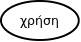
\includegraphics{images/use_case_case.png}}
     & Περίπτωση χρήσης. Περιγράφει τις δυνατές αλληλεπιδράσεις με το σύστημα \cite{virvou_uml}. \\ \hline

     \vspace{0.3cm}
     \center
     \resizebox*{0.20\textwidth}{!}{
     
\includegraphics{images/use_case_communication.png}}
     & Η σχέση <<communicates>>. Η σχέση αυτή ορίζεται μεταξύ περιπτώσεων χρήσης και σημαίνει ότι ένα στιγμιότυπο της πηγής (περίπτωσης χρήσης) συμπεριλαμβάνει τη συμπεριφορά του στόχου (περίπτωση χρήσης) \cite{virvou_uml}. \\ \hline

     \vspace{0.3cm}
     \resizebox*{0.20\textwidth}{!}{
     
\includegraphics{images/use_case_extend.png}}
     & Η σχέση <<extend>>. Δείχνει προαιρετική συμπεριφορά μίας περίπτωση χρήσης \cite{virvou_uml}. \\ \hline

     \vspace{0.3cm}
     \resizebox*{0.20\textwidth}{!}{
     
\includegraphics{images/use_case_include.png}}
     & Η σχέση <<include>>. Χρησιμοποιείται για να δείξει λειτουργικότητα που τη μοιράζονται πολλές περιπτώσεις χρήσης \cite{virvou_uml}. \\ \hline

     \vspace{0.3cm}
     \resizebox*{0.20\textwidth}{!}{
     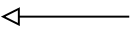
\includegraphics{images/use_case_generalization.png}}
     & Η γενίκευση περιπτώσεων χρήσης. Ο ειδικός ενεργοποιός κληρονομεί τις περιπτώσεις χρήσης του γενικού ενεργοποιού. Το βέλος πρέπει να δείχνει το γενικότερο ενεργοποιό. \cite{virvou_uml}. \\ \hline

     %\vspace{0.3cm}
     \center{
     \resizebox*{0.10\textwidth}{!}{
     
\includegraphics{images/use_case_boundary.png}}}
     & Τα όρια του συστήματος. \\ \hline

  \end{tabular}
\caption{Τα εικονίδια του διαγράμματος περιπτώσεων - χρήσης.}
\label{table:uml_use_case}
\end{center}
\end{table}



\begin{figure}
\begin{center}
\resizebox*{\textwidth}{!}{
\includegraphics{images/use_case_member.png}}
\caption{Διάγραμμα περιπτώσεων - χρήσης μέλους}
\label{fig:use_case_member}
\end{center}
\end{figure}

\begin{figure}
\begin{center}
\resizebox*{\textwidth}{!}{
\includegraphics{images/use_case_administrator.png}}
\caption{Διάγραμμα περιπτώσεων - χρήσης διαχειριστή}
\label{fig:use_case_administrator}
\end{center}
\end{figure}

\begin{figure}
\begin{center}
\resizebox*{\textwidth}{!}{
\includegraphics{images/use_case_ticket.png}}
\caption{Διάγραμμα περιπτώσεων - χρήσης αγοράς εισητηρίου}
\label{fig:use_case_ticket}
\end{center}
\end{figure}

\subsection{Διαγράμματα σειράς}

Τα διαγράμματα σειράς αναπαριστούν αλληλεπιδράσεις ανάμεσα στα αντικείμενα από μία χρονική άποψη. Η αναπαράσταση επικεντρώνεται στην έκφραση των αλληλεπιδράσεων. Οι συμβολισμοί που χρησιμοποιούνται στα διαγράμματα σειράς φαίνονται στον πίνακα \ref{table:uml_sequence}.

\begin{table}
\begin{center}
  \begin{tabular}{|m{0.20\textwidth}|m{0.60\textwidth}|}
    \hline
     \vspace{0.3cm}
     \resizebox*{0.20\textwidth}{!}{
     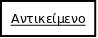
\includegraphics{images/sequence_object.png}}
     & Αντικείμενο. Ένα αντικείμενο αναπαριστάται με ένα ορθογώνιο και μία κάθετη γραμμή, που καλείται γραμμή ζωής του αντικειμένου \cite{virvou_uml}. \\ \hline

     %\vspace{0.3cm}
     \center{
     \resizebox*{!}{0.20\textwidth}{
     
\includegraphics{images/sequence_lifeline.png}}}
     & Ενεργοποίηση αντικειμένου. Μία ενεργοποίηση ανταποκρίνεται στο χρόνο κατά την διάρκεια του οποίου ένα αντικείμενο εκτελεί μία ενέργεια, είτε απευθείας ή μέσω άλλου αντικειμένου, που το χρησιμοποιεί σαν ημισυμβαλλόμενο. Οι ενεργοποιήσεις αναπαριστώνται με ορθογώνιες ράβδους, που τοποθετούνται κατά μήκος των γραμμών ζωής. Η αρχή και το τέλος μίας ράβδου ανταποκρίνεται αντίστοιχα στην αρχή και το τέλος μίας ενεργοποίησης \cite{virvou_uml}. \\ \hline

     \vspace{0.3cm}
     \resizebox*{0.20\textwidth}{!}{
     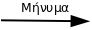
\includegraphics{images/sequence_message.png}}
     & Συγχρονισμένο Μηνύματα. Τα αντικείμενα επικοινωνούν ανταλλάσσοντας μηνύματα, τα οποία αναπαριστώνται με οριζόντια βέλη σχεδιασμένα από τον αποστολέα του μηνύματος προς τον παραλήπτη του μηνύματος \cite{virvou_uml}. Επειδή είναι συγχρονισμένα, θα πρέπει να περιμένει να τελειώσει η διαδικασία πριν προχωρήσει στην επόμενη \\ \hline

     \vspace{0.3cm}
     \resizebox*{0.20\textwidth}{!}{
     
\includegraphics{images/sequence_return.png}}
     & Επιστροφή. Βέλος επιστροφής μηνύματος. \\ \hline

  \end{tabular}
\caption{Τα εικονίδια του διαγράμματος σειράς.}
\label{table:uml_sequence}
\end{center}
\end{table}

Οι πιο σημαντική αλληλεπίδραση του πληροφοριακού μας συστήματος είναι η αγορά των εισιτηρίων και γι` αυτό το λόγο αναπαριστάται και σε διάγραμμα σειράς. Όπως φαίνεται και στο διάγραμμα σειράς στο σχήμα \ref{fig:sequence_ticket} ο πελάτης για να κλείσει το εισιτήριο του θα πρέπει πρώτα να συνδεθεί με το πληροφοριακό σύστημα. Έπειτα επιλέγει την ταινία που θέλει να δει και τον κινηματογράφο στον οποίο θέλει να την δει. Αφού ολοκληρωθούν με επιτυχία τα παραπάνω επιλέγει τις θέσεις, αφού πρώτα κάνει έλεγχο για την διαθεσιμότητα τους. Ολοκληρώνοντας τα παραπάνω, όλα τα στοιχεία περνάνε και στην φόρμα παραγγελίας 

\begin{landscape}
\begin{figure}
\begin{center}
\resizebox*{!}{\textwidth}{
\includegraphics{images/sequence_ticket.png}}
\caption{Διάγραμμα σειράς για την αγορά εισητηρίου}
\label{fig:sequence_ticket}
\end{center}
\end{figure}
\end{landscape}

\subsection{Διάγραμμα Βασικών κλάσεων πεδίου Εφαρμογής}

%\begin{landscape}
\begin{figure}
\begin{center}
\resizebox*{!}{\textwidth}{
\includegraphics{images/class_diagramm.jpg}}
\caption{Το διάγραμμα κλάσεων}
\label{fig:class_diagramm}
\end{center}
\end{figure}
%\end{landscape}


\subsection{Αναλυτικά διαγράμματα κλάσεων συνοδευμένα από OCL περιορισμούς}

\subsection{Διαγράμματα Επικοινωνίας και Αλληλεπίδρασης}




%ΔΕΝ ΧΡΕΙΑΖΟΝΤΑΙ
%\section{Μοντέλο Οντοτήτων-Συσχετίσεων της Βάσεις Δεδομένων του Πληροφοριακού Συστήματος}

%Στην ενότητα αυτή δίνεται η περιγραφή του μοντέλου Οντοτήτων-Συσχετίσεων (αγγλ. \en{Entity-Relationship Diagram} από το οποίο υλοποιείται το Σχεσιακό Διάγραμμα της Βάσης Δεδομένων του Πληροφοριακού Συστήματος.

%\subsection{Περιγραφή Οντοτήτων}
%\label{entity}

%Οι βασικές οντότητες είναι οι παρακάτω:

%\begin{description}
%\item test
%\end{description}

%\subsection{Περιγραφή Σχέσεων}
%\label{relationship}

%Οι βασικές σχέσεις είναι οι παρακάτω:

%\subsection{ER διάγραμμα του Πληροφοριακού Συστήματος}

%Οι ενότητες \ref{entity} και \ref{relationship} απεικονίζονται στο σχήμα \ref{}.






\phantomsection \label{Βιβλιογραφία}
\addcontentsline{toc}{section}{Βιβλιογραφία}
%\mtcaddchapter[Βιβλιογραφία] % Λόγω του minitoc
\bibliographystyle{plain}
\bibliography{references}

\newpage

\end{document}

